\section[对权重的依赖]{对权重的依赖\\Dependency on the Weights}
一个已经获得最小二乘问题基本知识的人很快提出这个问题:权重有多重要? 如果我们改变他们有点多少,这改变了解决方案? 让我们试着得到一些洞察的问题。 像往常一样,我们从一组观测方程$ A\textbf{\textit{x}}=\textbf{\textit{b}}-\textbf{\textit{e}} $和权重矩阵$C$开始。

我们将观察向量$\textbf{\textit{b}}$分成两个子向量。首先,我们对$\textbf{\textit{b}}_{1}$和$\textbf{\textit{b}}_{2}$的尺寸没有限制。向量$\textbf{\textit{e}}$和矩阵$A$和权重$C$
\begin{align*}
\textbf{\textit{b}}=
\begin{bmatrix}
\textbf{\textit{b}}_{1} \\	
\textbf{\textit{b}}_{2}
\end{bmatrix},
\quad
\textbf{\textit{e}}=
\begin{bmatrix}
\textbf{\textit{e}}_{1} \\	
\textbf{\textit{e}}_{2}
\end{bmatrix},
\quad
A=
\begin{bmatrix}
A_{1} \\	
A_{2}
\end{bmatrix},
\quad
C=
\begin{bmatrix}
C_{1} & 0\\	
0   & C_{2}
\end{bmatrix}.
\end{align*}
这意味着在两组观察之间没有权重耦合。原来的问题变成两个明显的问题:
\begin{align*}
A_{1}\textbf{\textit{x}}&=\textbf{\textit{b}}_{1}-\textbf{\textit{e}}_{1}  &\text{权阵} \ C_{1}                      \\
A_{2}\textbf{\textit{x}}&=\textbf{\textit{b}}_{2}-\textbf{\textit{e}}_{2}  &\text{权阵} \ C_{2}    
\end{align*}
并且我们可以计算每个系统的解。现在有趣的问题是:这些解决方案与整个问题的解决方案相比有什么表现?

我们将看到当我们将第二组的权重$C_{2}$改变为$ C_{2}+\delta C_{2}$时,解$\hat{\textbf{\textit{x}}}$的误差$ \delta \textbf{\textit{x}} $是多少。$ \delta \textbf{\textit{x}} $的表达式涉及一个有用矩阵公式的矩阵计算。原始问题的正规方程是
\begin{align*}
\begin{bmatrix}
A^{T}_{1} &	A^{T}_{2}
\end{bmatrix}
\begin{bmatrix}
C_{1} &	0 \\
0     &	C_{2}
\end{bmatrix}
\begin{bmatrix}
A_{1} \\
A_{2}
\end{bmatrix}  \hat{\textbf{\textit{x}}} = 
\begin{bmatrix}
A^{T}_{1} &	A^{T}_{2}
\end{bmatrix}
\begin{bmatrix}
C_{1} &	0 \\
0     &	C_{2}
\end{bmatrix}
\begin{bmatrix}
\textbf{\textit{b}}_{1} \\
\textbf{\textit{b}}_{2}
\end{bmatrix}.
\end{align*}
这可以写成
\begin{align}
(A^{T}_{1}C_{1}A_{1}+A^{T}_{2}C_{2}A_{2})\hat{\textbf{\textit{x}}}=A^{T}_{1}C_{1}\textbf{\textit{b}}_{1}+A^{T}_{2}C_{2}\textbf{\textit{b}}_{2}.
\end{align}
注意如何收集来自两个问题的正规方程。对正态方程的贡献具有可加性特征。扰动的问题是
\begin{align}
(A^{T}_{1}C_{1}A_{1}+A^{T}_{2}(C_{2}+\delta C_{2} )A_{2})(\hat{\textbf{\textit{x}}}+\delta \textbf{\textit{x}} )=(A^{T}_{1}C_{1}\textbf{\textit{b}}_{1}+A^{T}_{2}(C_{2}+\delta C_{2} )\textbf{\textit{b}}_{2}).
\end{align}
现在从(6.32)中减去(6.31),得到$ \delta \textbf{\textit{x}} $的方程:
\begin{align}
(A^{T}_{1}C_{1}A_{1}+A^{T}_{2}(C_{2}+\delta C_{2} )A_{2})\delta \textbf{\textit{x}} + A^{T}_{2}\delta C_{2}A_{2}\textbf{\textit{x}}=
A^{T}_{2}\delta C_{2}\textbf{\textit{b}}_{2}.
\end{align}
我们令$ N= A^{T}_{1}C_{1}A_{1} + A^{T}_{2}C_{2}A_{2}$和$ \hat{\textbf{\textit{e}}}_{2} = \textbf{\textit{b}}_{2} - A_{2}\textbf{\textit{x}}  $。那么$\hat{\textbf{\textit{x}}}$的变化是
\begin{align}
\delta \textbf{\textit{x}} = ( N + A^{T}_{2}\delta C_{2}A_{2})^{-1}
A^{T}_{2}\delta C_{2} \hat{\textbf{\textit{e}}}_{2}.
\end{align}
下面的重要公式,取自(8.45),得出:
\begin{align}
( N + A^{T}_{2}\delta C_{2}A_{2})^{-1} = N^{-1} - N^{-1}A^{T}_{2}
(A_{2}N^{-1}A^{T}_{2} +(\delta C_{2})^{-1} )^{-1} A_{2} N^{-1}
\end{align}
对于$n$个观测值,该矩阵乘以$ A^{T}_{2}\delta C_{2} \hat{\textbf{\textit{e}}}_{2} $得到$ \delta \textbf{\textit{x}} $。如果我们专注于一个单一的观测值,$ A^{T}_{2} $成为一个$n$乘1矩阵, $ \delta C_{2} $是1乘1.我们命名$ A_{2}N^{-1}A^{T}_{2} = s $并且得到
\begin{align*}
\delta \textbf{\textit{x}} = N^{-1} A^{T}_{2} (1-\dfrac{\delta C_{2}}{1+s\delta C_{2}}s)\delta C_{2}\hat{e}_{2}
\end{align*}
或
\begin{align}
\delta \textbf{\textit{x}} = \dfrac{\hat{e}_{2}\delta C_{2} }{1+s\delta C_{2}}N^{-1}A^{T}_{2}.
\end{align}
表达式(6.36)揭示了几个有趣的事实。解决方案中的变化 $ \delta \textbf{\textit{x}} $(一阶近似)与权重变化$ \delta C_{2} $成正比。在与$A_{2}$中包含的观察相关的未知数中,$ \delta \textbf{\textit{x}} $变化最大。$ N^{-1}A^{T}_{2} $只有来自$N^{-1}$的列的贡献,该列对应于不同于零的$ A^{T}_{2} $。

已经在1823年C.F.高斯找到一个单一权重$ \delta C_{2} $的变化的类似表达式。参见高斯(1995)中的“更新观察变化的未知数”一节。

\begin{figure}[htb]
	\centering
	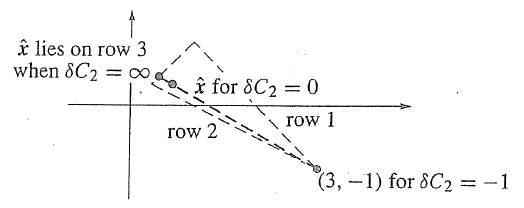
\includegraphics[width=0.7\linewidth]{TeX_files/Part02/chapter06/image/6-1}
	\caption{Dependence of $ \hat{\textbf{\textit{x}}}$ on $ \delta C_{2}$ \text{在实例} 6.4}
\end{figure}

实例6.4 \ 我们想要演示关于简单最小二乘问题的过程:
\begin{align*}
A = 
\begin{bmatrix}
1&1 \\	
1&2 \\		
-1&1 	
\end{bmatrix} \quad 
\text{和} \quad 
\textbf{\textit{b}}=
\begin{bmatrix}
2 \\	
1 \\		
0 	
\end{bmatrix} \quad 
\text{和} \quad 
C+\delta C_{2} =
\begin{bmatrix}
1   &   & \\	
&   2   & \\		
&   &  1+\delta C_{2} 	
\end{bmatrix} 
\end{align*}
然后$ \delta C_{2} =0 $照常产生解$\hat{\textbf{\textit{x}}}$和残差向量$\hat{\textbf{\textit{e}}}$:
\begin{align*}
\hat{\textbf{\textit{x}}} = \dfrac{1}{3}
\begin{bmatrix}
2 \\	
1 	
\end{bmatrix} \quad 
\text{和} \quad 
\hat{\textbf{\textit{e}}} = \dfrac{1}{3}
\begin{bmatrix}
3 \\	
-1 \\
1	
\end{bmatrix}.
\end{align*}
令$\delta C_{2} =-1 $对应于消除第三观测量。然后$ \hat{\textbf{\textit{x}}}=(3,-1)$是前两行的交点。我们得到第三行元素从(3,-1)到(5/11,5/11)的线段,随着$\delta C_{2} $从-1到$ \infty$。所有权重变化,我们显然可以在三角形内的任何地方获得解。

 $M$文件$dw$反映了发生了什么。
 
 这种权重变化的方法对于少量的观测是极好的。对于一个更大的问题的更多的定性知识,我们转向一个更强大的工具。

现在我们要求更多的定量结果:如果权重改变,投影$\textbf{\textit{p}}=P\textbf{\textit{b}}$在$A$的列空间中移动多少?这种运动的描述是
\begin{align}
tan \alpha = \dfrac{\rVert \textbf{\textit{p}}_{2} - \textbf{\textit{p}}_{1}\rVert c_{1}}{\rVert \textbf{\textit{b}} - \textbf{\textit{p}}_{1}\rVert c_{1}}.
\end{align}
范数由$ \rVert \textbf{\textit{x}} \rVert c_{1}  = \rVert  C_{1}\textbf{\textit{x}} \rVert$加权,$ \alpha$是在行程$ \overline{\textbf{\textit{p}}_{1}\textbf{\textit{p}}_{2}}$处的$\textbf{\textit{b}}$角度。注意图6.2是在$C_{1}$范数中绘制的。在$\textbf{\textit{p}}_{2}$处的角度为$C_{2}$正交;但在$C_{1}$范数中的角度是$ \dfrac{\pi}{2} - \alpha$。从$C_{1}$到$C_{2}$范数的变化导致角度从$ \dfrac{\pi}{2}$改变到$ \dfrac{\pi}{2} - \alpha$。

矩阵$C$的平方根$W$是满足$W^{2}=C$的正定矩阵。这样的矩阵肯定存在,是唯一的,并且非奇异。我们定义$ D = W^{-1}_{1}C_{2}W^{-1}_{1}$,其条件数$c(D)$最大和最小特征值之间的比率可以与角度$ \alpha$相关:
\begin{align}
2\lvert tan\alpha \rvert \leq \sqrt{c(D)} - \dfrac{1}{\sqrt{c(D)}}.
\end{align}

\begin{figure}[!h]
	\centering
	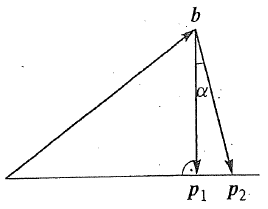
\includegraphics[height=0.23\linewidth]{TeX_files/Part02/chapter06/image/6-2}
	\caption{投影与范数之间的关系. 图是在 $C_{1}$的范数下画的.}
\end{figure}

让我们重复一下:最小二乘问题由系数矩阵$A$,权重$C_{0}$和观测值$\textbf{\textit{b}}$给出。我们考虑所有权重矩阵$C$,使得$ W^{-1}_{0}CW^{-1}_{0}$的特征值位于封闭区间$[s,t]$中。在$C_{0}$的范数中总是找到
\begin{align}
\lvert tan \alpha \rvert \leq \dfrac{1}{2} (\sqrt{\dfrac{t}{s}} - \sqrt{\dfrac{s}{t}}).
\end{align}
角度$ \alpha$测量从$\textbf{\textit{b}}$看到的最小二乘结果的位移。存在至少一个矩阵$C$,其等式符号是有效的。此外,对应于$C_{1}$和$C_{2}$的残差向量的范数之间的比率被限制
\begin{align}
\dfrac{1}{\sqrt{\lambda_{max}}} \leq \dfrac{\rVert \textbf{\textit{b}} - \textbf{\textit{p}}_{1}\rVert c_{1}}{\rVert \textbf{\textit{b}} - \textbf{\textit{p}}_{2}\rVert c_{2}} \leq \sqrt{\lambda_{max}}
\end{align}
其中 $ \lambda_{max}$是该矩阵$ W^{-1}_{2}CW^{-1}_{2}$的最大特征值。

关于最小二乘问题中权重变化的主要结果引自Krarup(1972)。条件数是主要的问题。如果条件数很大,忽略观测值之间可能的相关性的效果可能是危险的。

示例6.5 \ 我们引入具有强相关性的$n$乘$n$的协方差矩阵:
\begin{align*}
\Sigma_{b} =
\begin{bmatrix}
2    &    -1          &        &        & \\
-1   &     2    &    -1        &        & \\
&       \ddots  &  \ddots      & \ddots & \\
&          &         -1    &   2    &  -1 \\
&          &          &       -1    &   2
\end{bmatrix}.
\end{align*}
它的逆具有特殊的形式
\begin{align*}
D = C_{2} = \Sigma^{-1}_{b} =
\left\{
\begin{aligned}
\dfrac{i(n+1-j)}{n+1} \quad \text{for} \ i\leq j\\
\dfrac{j(n+1-i)}{n+1} \quad \text{for} \ i\geq j.
\end{aligned}
\right.
\end{align*}
特征值是$ 4sin^{2} \dfrac{i\pi}{2(n+1)}$,所以条件是$ c(D) \approx \dfrac{4(n+1)^{2}}{\pi^{2}} < n^{2} $。由(6.39)
\begin{align*}
\lvert tan \alpha \rvert \leq \dfrac{1}{2} ( \sqrt{c(D)} - \dfrac{1}{\sqrt{c(D)}}) \approx \dfrac{1}{\pi} (n+1) \rightarrow \infty.
\end{align*}
强相关可以使我们任意地远离对应于$C_{1}=I$的解。

示例6.6 \ 如果$ D = C_{2} = I +t\Sigma^{-1}_{b}$和$ t \approx 10^{-2}$,相关性较弱:
\begin{align*}
c(D) = \dfrac{1+4sin^{2}\dfrac{n\pi}{2(n+1)}}{1+4sin^{2}\dfrac{\pi}{2(n+1)}} \approx 
(1+4t)(1-4t\dfrac{\pi^{2}}{4n^{2}}) \approx 1+4t.
\end{align*}
\begin{align*}
\lvert tan \alpha \rvert \leq \dfrac{1}{2} (\sqrt{1+4t} - \dfrac{1}{\sqrt{1+4t}}) = \dfrac{2t}{\sqrt{1+4t}}.
\end{align*}
另外 $\lvert tan \alpha \rvert < 2t $.